%%%%%%%%%%%%%%%%%%%%%%%%%%%%%%%%%%%%%%%%%
% Journal Article
% LaTeX Template
% Version 1.4 (15/5/16)
%
% This template has been downloaded from:
% http://www.LaTeXTemplates.com
%
% Original author:
% Frits Wenneker (http://www.howtotex.com) with extensive modifications by
% Vel (vel@LaTeXTemplates.com)
%
% License:
% CC BY-NC-SA 3.0 (http://creativecommons.org/licenses/by-nc-sa/3.0/)
%
%%%%%%%%%%%%%%%%%%%%%%%%%%%%%%%%%%%%%%%%%

%----------------------------------------------------------------------------------------
%	PACKAGES AND OTHER DOCUMENT CONFIGURATIONS
%----------------------------------------------------------------------------------------

\documentclass[twoside]{article}
\usepackage{blindtext} % Package to generate dummy text throughout this template

\usepackage[sc]{mathpazo} % Use the Palatino font
\usepackage[T1]{fontenc} % Use 8-bit encoding that has 256 glyphs
\linespread{1.05} % Line spacing - Palatino needs more space between lines
\usepackage{microtype} % Slightly tweak font spacing for aesthetics
\usepackage{amsmath}
\usepackage{listings}
\usepackage{mathtools}
\usepackage[english]{babel} % Language hyphenation and typographical rules

\usepackage[hmarginratio=1:1,top=32mm,columnsep=20pt]{geometry} % Document margins
\usepackage[hang, small,labelfont=bf,up,textfont=it,up]{caption} % Custom captions under/above floats in tables or figures
\usepackage{booktabs} % Horizontal rules in tables

\usepackage{lettrine} % The lettrine is the first enlarged letter at the beginning of the text

\usepackage{enumitem} % Customized lists
\setlist[itemize]{noitemsep} % Make itemize lists more compact

\usepackage{abstract} % Allows abstract customization
\renewcommand{\abstractnamefont}{\normalfont\bfseries} % Set the "Abstract" text to bold
\renewcommand{\abstracttextfont}{\normalfont\small\itshape} % Set the abstract itself to small italic text

\usepackage{titlesec} % Allows customization of titles
\renewcommand\thesection{\Roman{section}} % Roman numerals for the sections
\renewcommand\thesubsection{\roman{subsection}} % roman numerals for subsections
\titleformat{\section}[block]{\large\scshape\centering}{\thesection.}{1em}{} % Change the look of the section titles
\titleformat{\subsection}[block]{\large}{\thesubsection.}{1em}{} % Change the look of the section titles

\usepackage{fancyhdr} % Headers and footers
\pagestyle{fancy} % All pages have headers and footers
\fancyhead{} % Blank out the default header
\fancyfoot{} % Blank out the default footer
% \fancyhead[C]{Running title $\bullet$ May 2016 $\bullet$ Vol. XXI, No. 1} % Custom header text
\fancyfoot[C]{\thepage} % Custom footer text

\usepackage{titling} % Customizing the title section

\usepackage{hyperref} % For hyperlinks in the PDF

%----------------------------------------------------------------------------------------
%	TITLE SECTION
%----------------------------------------------------------------------------------------

\setlength{\droptitle}{-4\baselineskip} % Move the title up

\pretitle{\begin{center}\Huge\bfseries} % Article title formatting
\posttitle{\end{center}} % Article title closing formatting
\title{Guidelines for Camera Profiling} % Article title
\author{%
    \textsc{Thatcher Freeman} \\[1ex] % Your name
    \normalsize \href{https://github.com/thatcherfreeman}{github.com/thatcherfreeman}
}
\date{}%\today} % Leave empty to omit a date
\renewcommand{\maketitlehookd}{%
    \begin{abstract}
    \noindent Camera color spaces are characterized by an OETF, a function mapping light values to code values, and by a color gamut, specified by the CIE x,y chromaticity of the red, green, blue, and white point. These can be estimated with a set of images constructed in the right conditions and this document will illustrate how to best capture these images.
    \end{abstract}
}

%----------------------------------------------------------------------------------------

\begin{document}

% Print the title
\maketitle

%----------------------------------------------------------------------------------------
%	ARTICLE CONTENTS
%----------------------------------------------------------------------------------------
\tableofcontents

\section{Prerequisites}
To integrate a camera into a color managed pipeline, the camera must be profiled with a selected color space, ISO, and lens selection. Assuming you have already selected a scene-referred in-camera color space based on a maximization of dynamic range and a minimzation of banding artifacts under a given bit-depth, the remaining choices that will impact the profiling will be the choice of ISO and lens.

\subsection{ISO Selection}
For camera profiling, you should select an ISO that maximizes dynamic range (the ``Native'' ISO from the spec sheet, or the lowest, non-extended ISO). If you more commonly shoot at a different ISO, you could choose to also profile the preferred alternate ISO. The concern is that some cameras change their log curve depending on the choice of ISO, so if your camera does not do this, then the Native ISO is the ideal choice for profiling.

\subsection{Lens Selection}
Every piece of glass will impart a subtle tint on the image that the camera sees and this will therefore affect the camera's measured color primaries and the overall gamut profiling step. If the camera profiling is intended to be versatile and work for all footage shot on a camera model, then a neutrally colored lens with no filtration should be used. If you're making a camera profile for a specific project with known lenses and filtration, then those lenses should be selected for this process, with the expected filtration.

\newpage \section{Summary List of Shots}
This whole process will require you to take the following images, ideally in the form of video clips that are about 1 second long:

\subsubsection*{OETF Profiling}
\begin{enumerate}
    \item[1.] Exposure bracket of a scene with at least 8 exposures, one stop apart.
    \item[2.] Image with the lens cap on
    \item[3.] Image that shows the clipping point
    \item[4.] Image that shows a proper exposure of middle gray
\end{enumerate}

\subsubsection*{Gamut Profiling}
\begin{enumerate}
    \item[5.] Shot of a Macbeth color chart under an incadescent light
    \item[6.] Shot of a grey or white card under the same incadescent light
    \item[7.] Shot of a Macbeth color chart under direct sunlight
    \item[8.] Shot of a grey or white card in the same direct sunlight
\end{enumerate}

\newpage
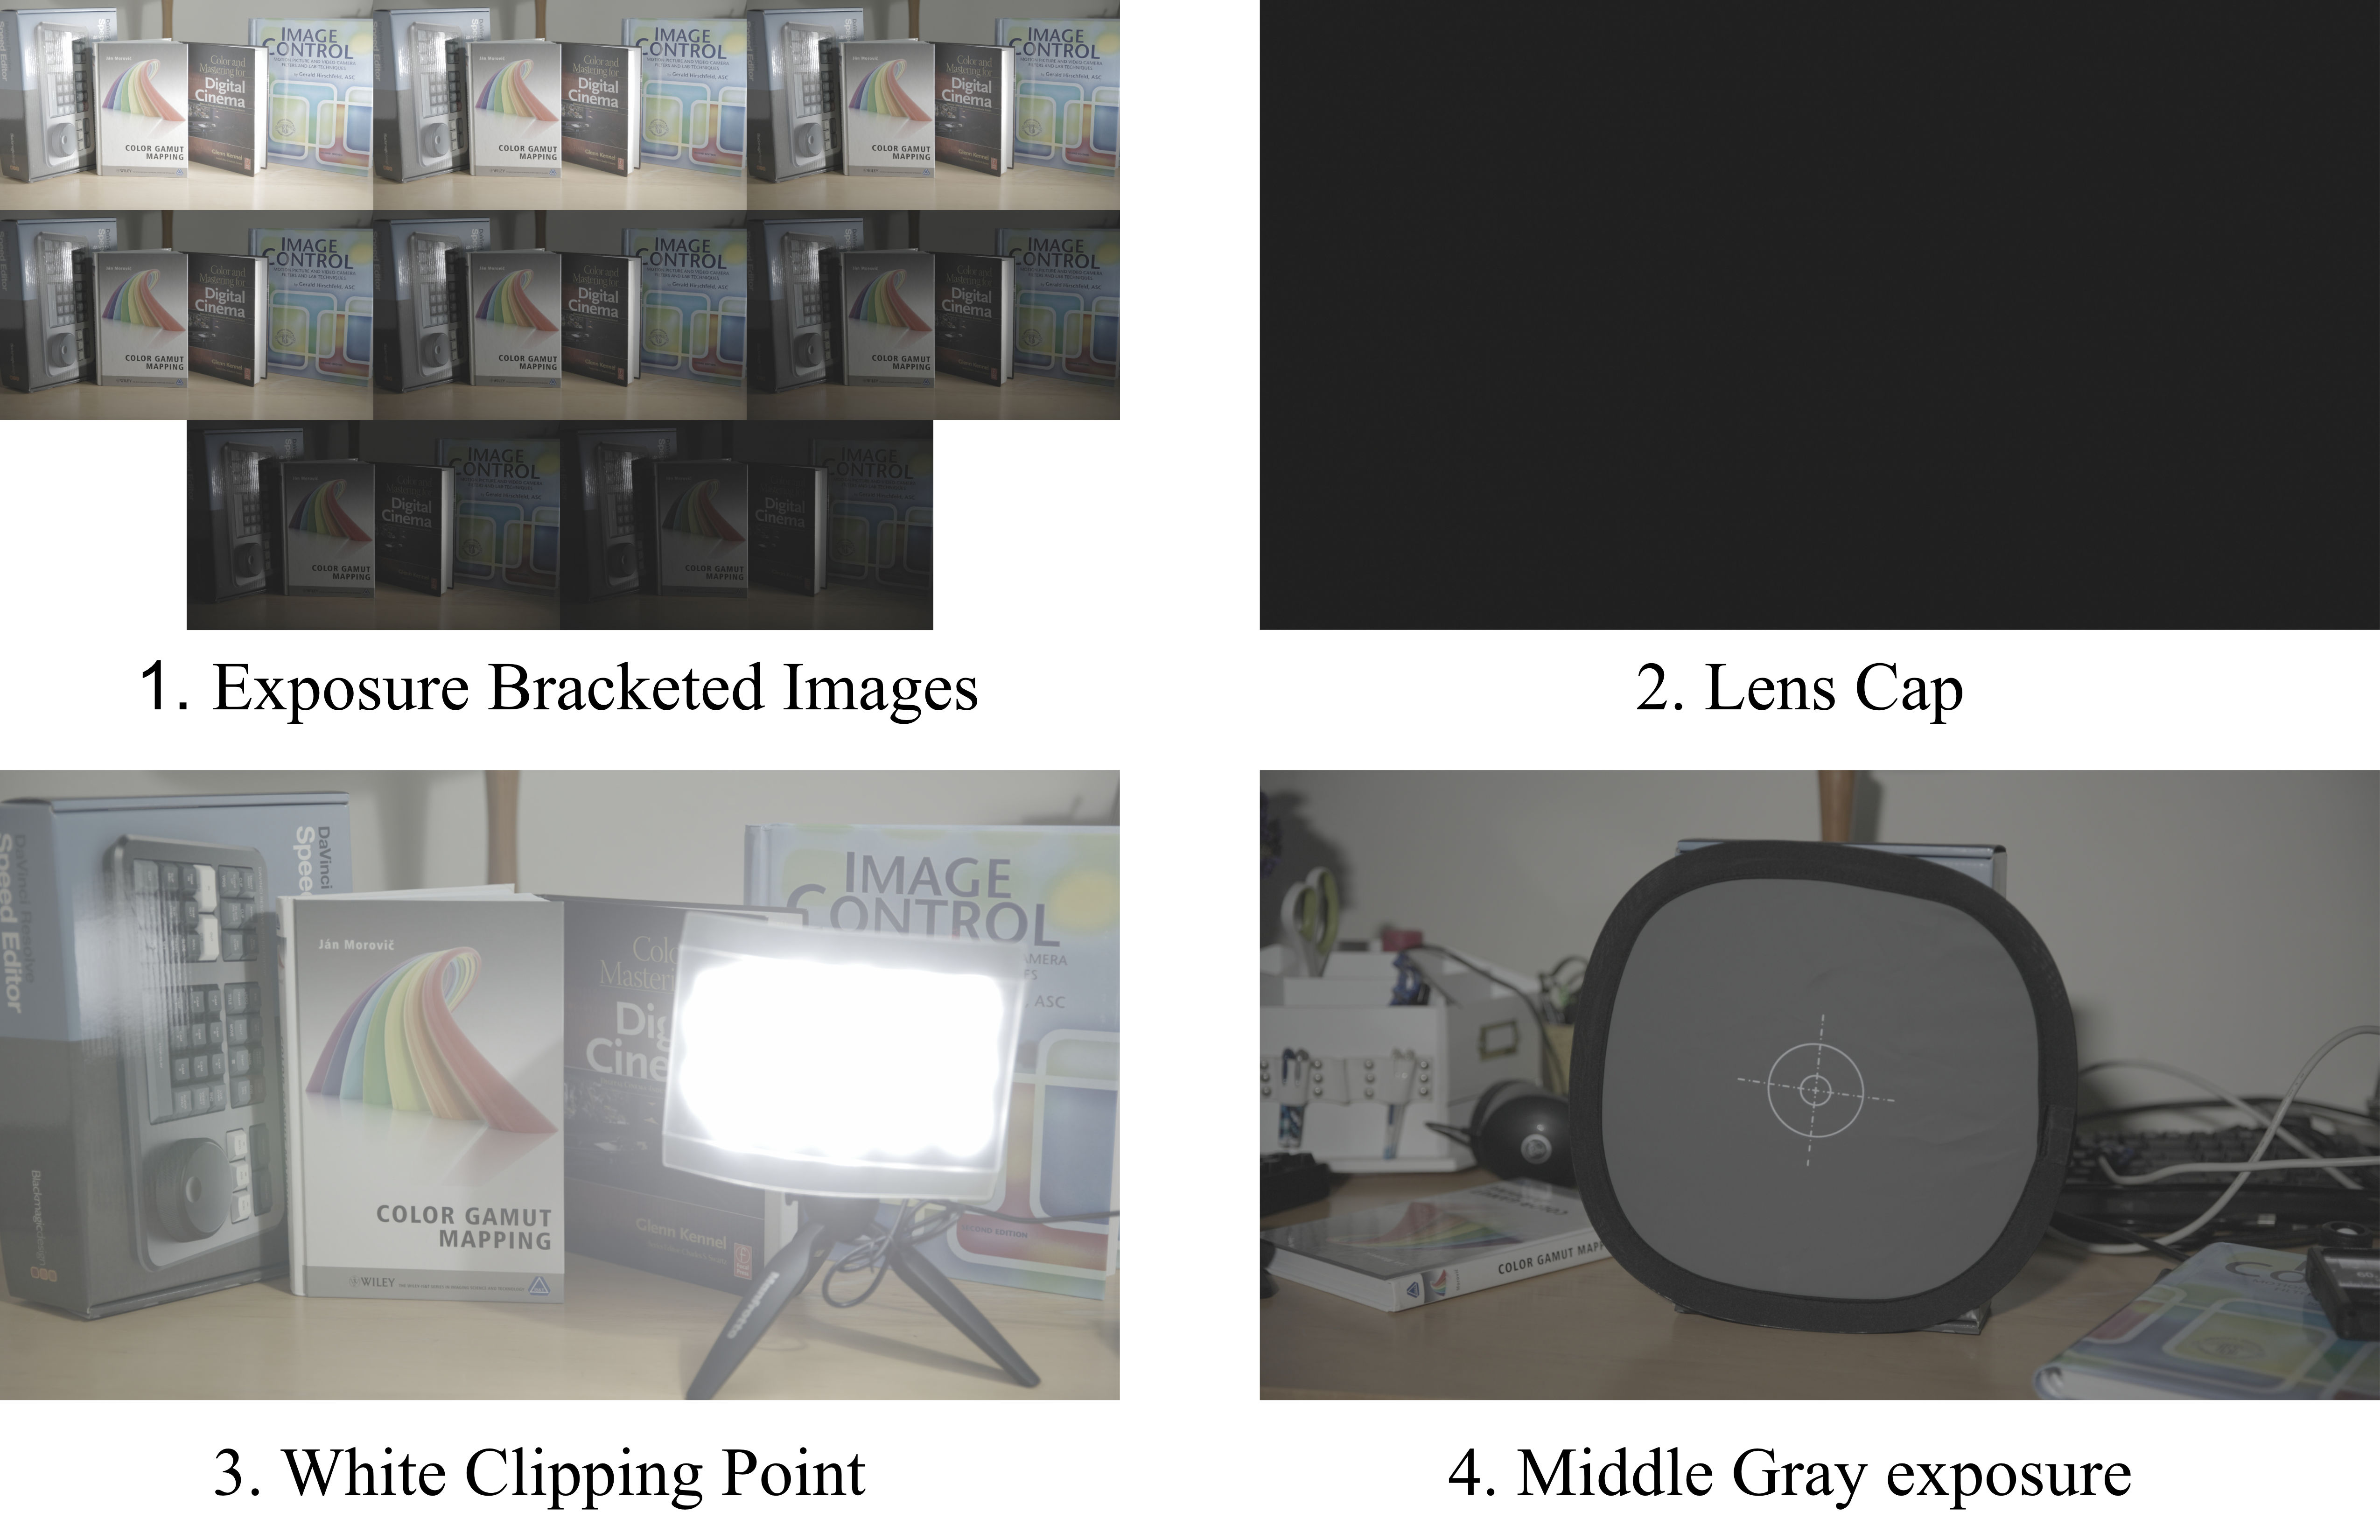
\includegraphics[scale=0.35]{images/OETF Images.jpg}

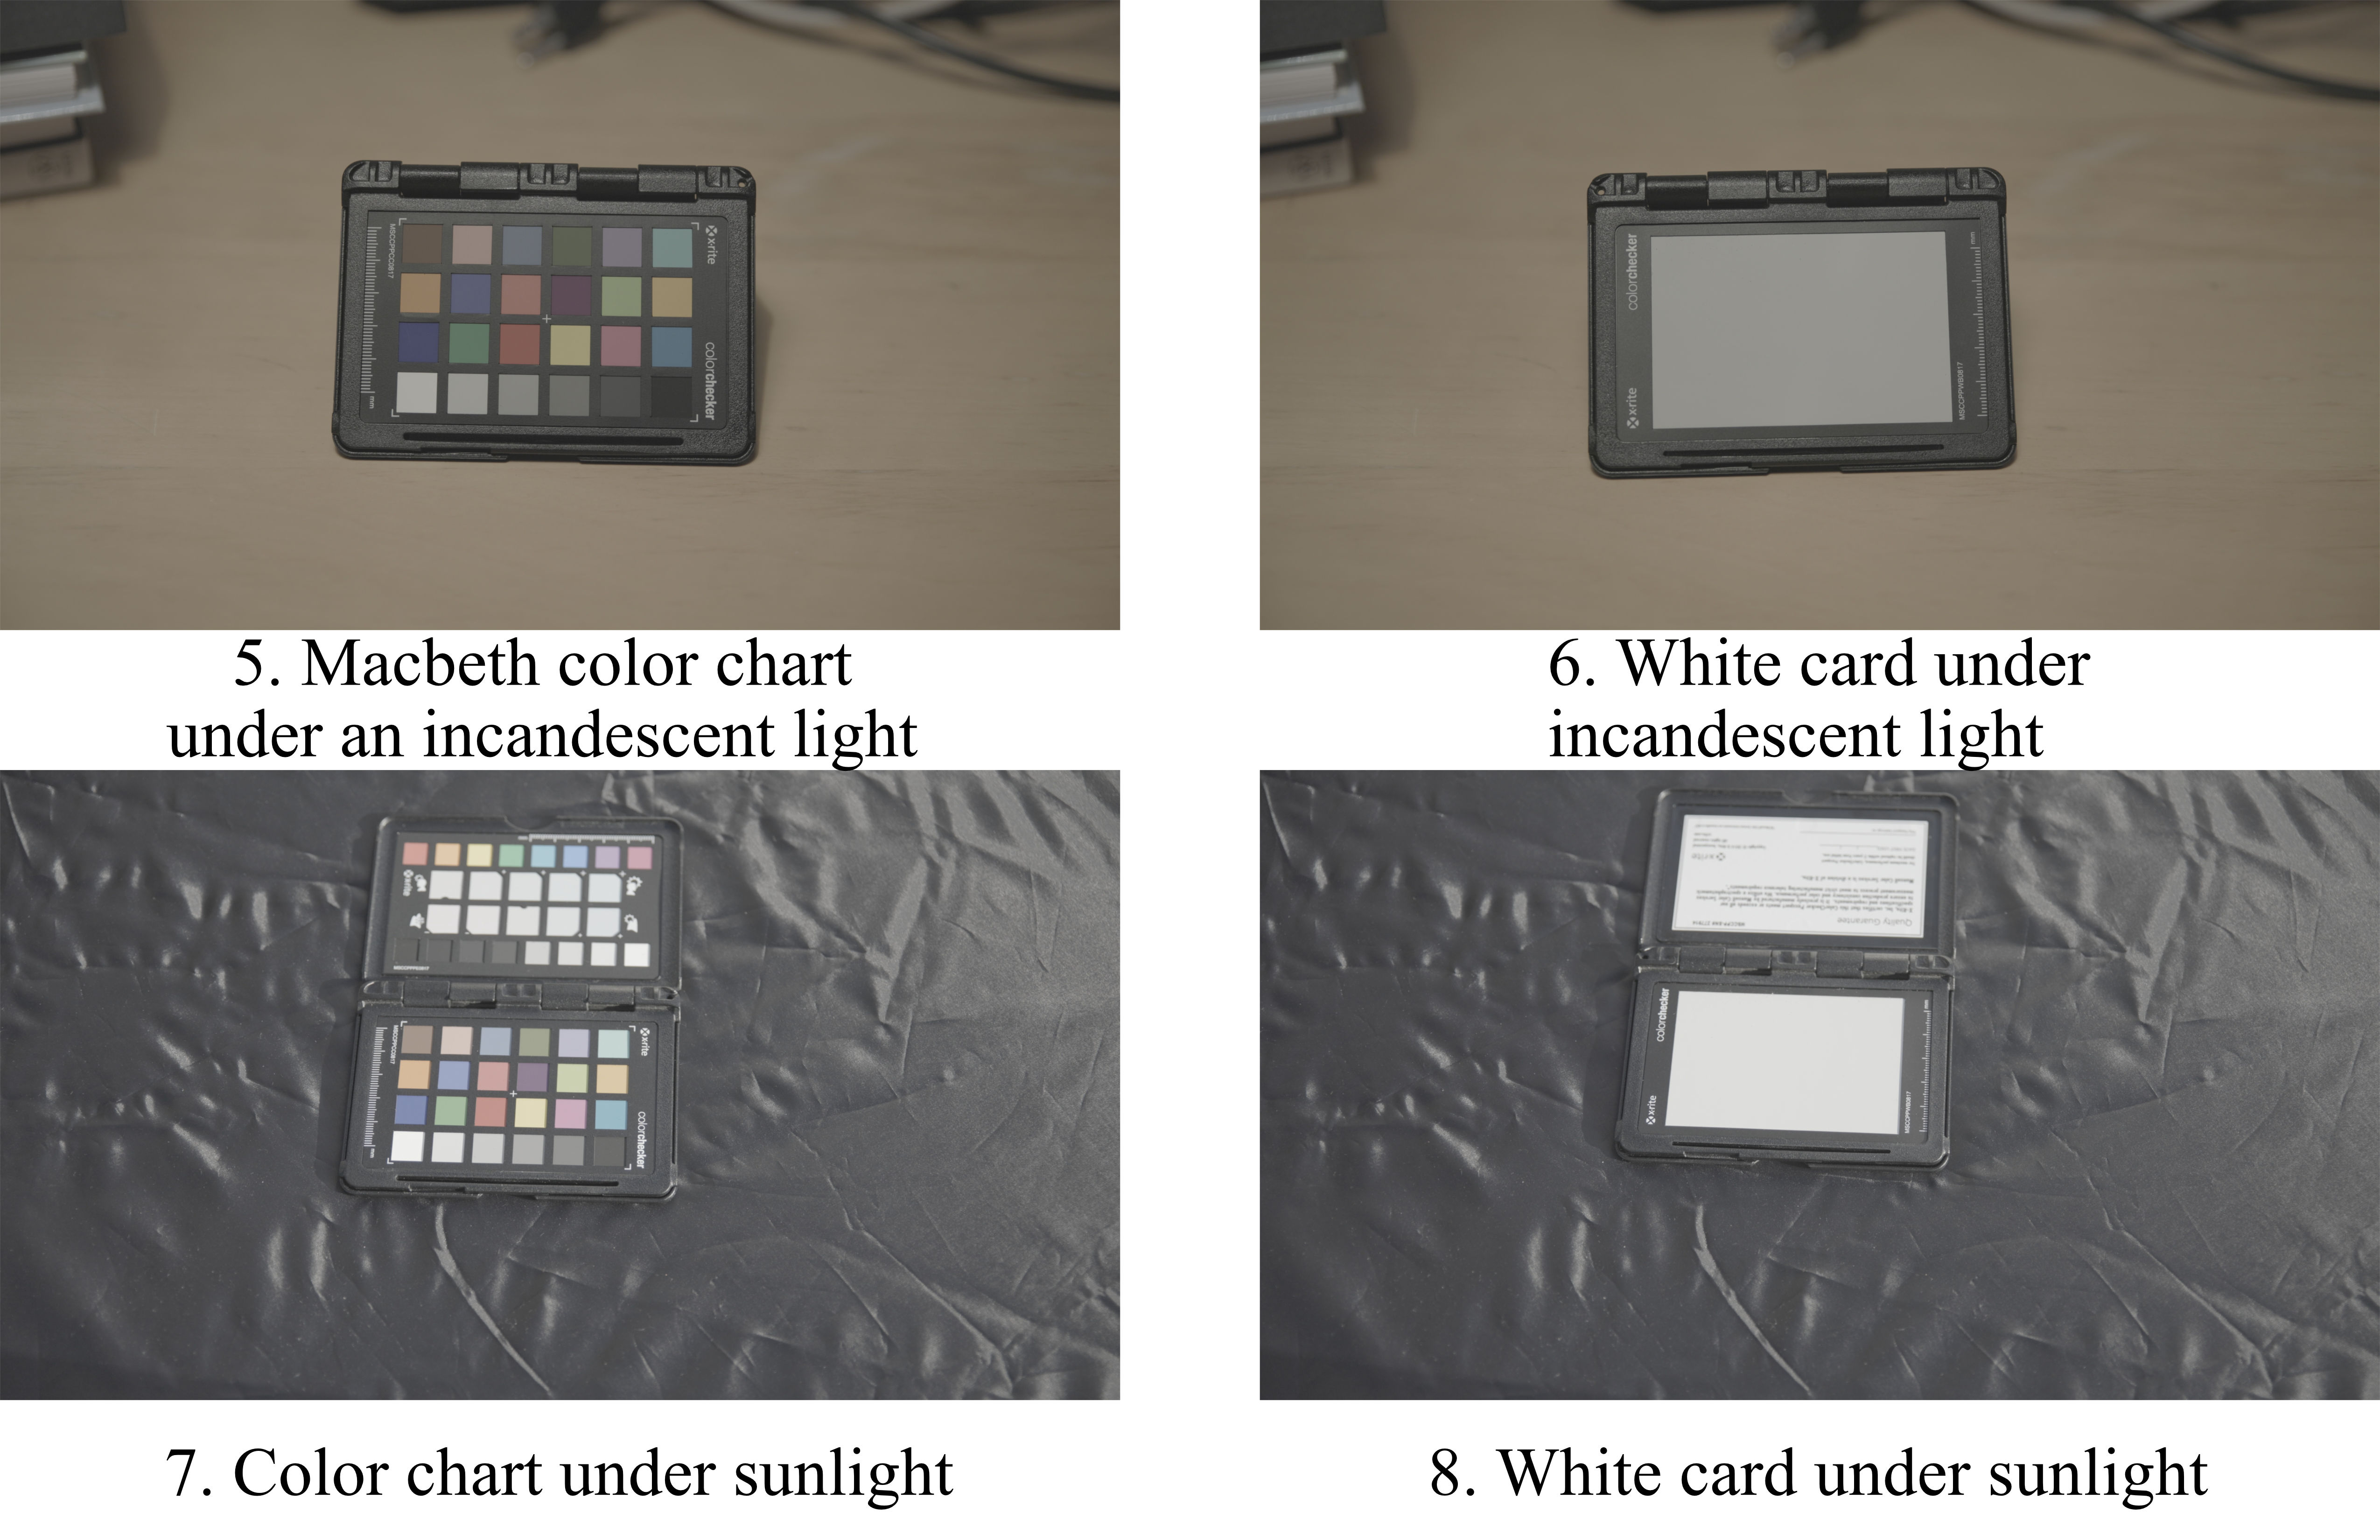
\includegraphics[scale=0.35]{images/Gamut Images.jpg}


\newpage\section{Images for OETF Profiling}
The first step in profiling a camera is to be capable of linearizing the image. This requires inverting the camera OETF and therefore obtaining the ability to map from the image code values to a quantity of photons that the camera saw. Once we have transformed an image to scene-linear, we obtain the ability to convert to other color spaces, to exposure match images shot with different exposure settings, and to apply gamut transformations. Thus, this is a prerequisite to Gamut Profiling. \\

\subsection{Exposure Bracketing}

\subsubsection{Procedure}
The first group of images needed are an exposure bracket. The camera will be fixed in position on a tripod, pointed at a stationary scene with fixed lighting so that all images align. The camera will be set with a slow shutter speed (360 degree shutter angle) and exposed for a second. Then, the shutter angle will be stopped down one stop at a time and new shots will be taken until the camera does not allow any further reduction in exposure. There should be no change to ISO, Aperture, White Balance, Lens, Focus Distance, or quantity of light across the exposure bracket. \\

The choice of scene is relatively flexible and should be achievable by shooting a bookshelf or a living room under controlled lighting. \\

\begin{figure}[h]
    \centering
    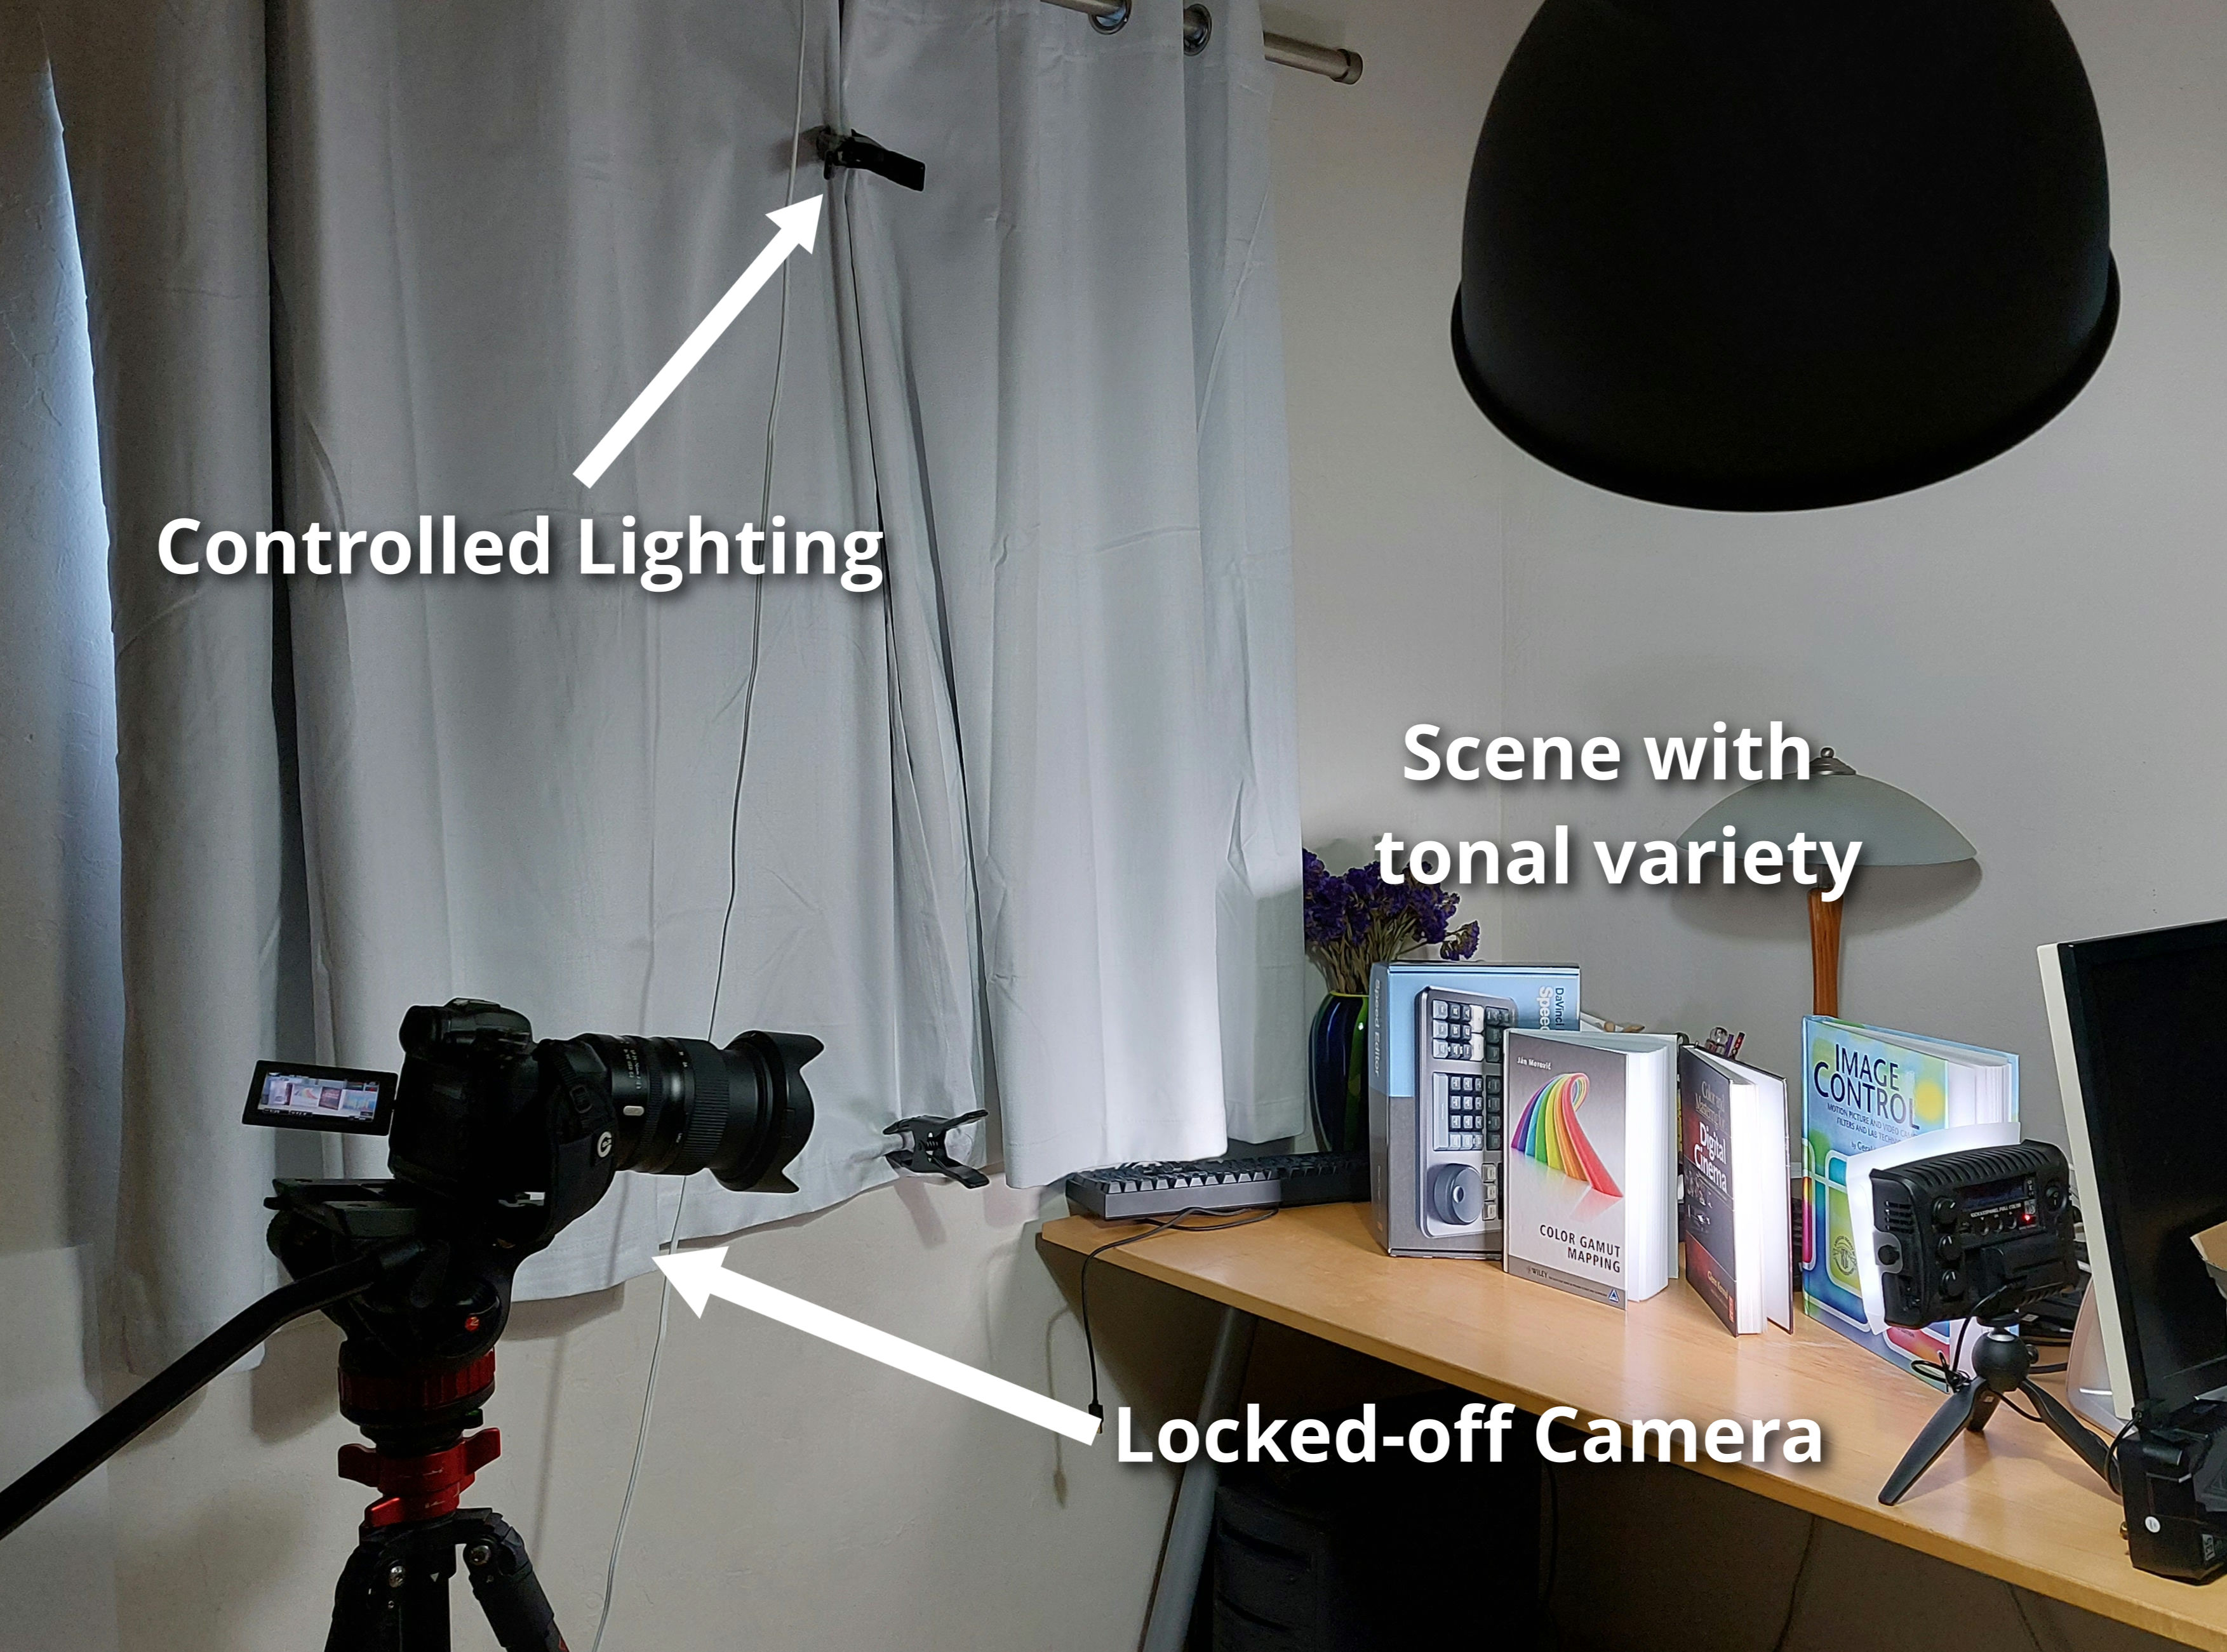
\includegraphics[scale=0.1]{images/exposure_bracket_setup0000.jpg}
\end{figure}


\subsubsection{Scene Requirements}
\begin{enumerate}
    \item \textbf{A stationary subject} - The captured images will need to be aligned, so the scene cannot move over the course of capturing the exposures.
    \item \textbf{Controlled lighting} - Lighting should be done artificially so that the moving sun, cloud coverage, or other variations in light quantity and direction are not a factor. The light should remain unchanged in position and intensity for the entire exposure ramp.
    \item \textbf{Adequate quantity of light} - There should be enough light that there are some clipped pixels in the brightest exposure. The brightest exposure should be such that there aren't gaps between the clipping point and the tonal mass.
    \item \textbf{Tonal Variety} - There should be a wide variety of tones in the scene rather than just a few monotonal patches in a test chart, or large blocks of shadows.
\end{enumerate}

\subsubsection{Scene Non-Requirements}
\begin{enumerate}
    \item \textbf{Color Charts} - For OETF profiling, we do not need the image to have any sort of test chart in it.
    \item \textbf{High quality lighting} - The quality of the light is irrelevant for this part of the process, so feel free to choose a light based on the quantity of output rather than by how it matches some standard illuminant.
\end{enumerate}

\subsubsection{Camera Requirements}
\begin{enumerate}
    \item \textbf{Clipping in first exposure} - The brightest exposure has some clipped pixels in it, so we can make sure we've covered the top of the tonal range.
    \item \textbf{Darkest Exposure is near-black} - The darkest exposure out of the set should be buried in the shadows so the bottom end of the OETF can be profiled.
    \item \textbf{ND filters are NOT used} - Neutral Density filters should not be added to aid in decreasing the exposure
    \item \textbf{The camera is stationary} - The camera should be locked off on a tripod so all exposures in the bracket are aligned.
    \item \textbf{Fixed WB, ISO, Aperture, Lens, and Focus} - These settings should all be fixed so the images will be directly comparable.
    \item \textbf{Image stabilization is turned off} - This is to reduce the risk that the images become misaligned due to randomness in the sensor or lens element positions.
\end{enumerate}

\subsubsection{Camera Non-Requirements}
\begin{enumerate}
    \item \textbf{Correct White Balance} - This test does not require a specific ``correct'' white balance setting, but it does require that the camera's white balance does not change between exposures. It may be easiest to just set this to Daylight or to set a custom white balance for your specific scene. The choice does not matter.
\end{enumerate}


\subsection{Pure Black Image}
As a sanity check, we need to ensure that blacks aren't mapped to negative linear values. This will also help us identify if there is fixed pattern noise in the sensor of the camera that should be corrected during the profiling process.

\subsubsection{Procedure}
Put the lens cap on the lens and shoot a one-second clip with the same ISO used for the rest of this process.

\subsubsection{Requireemnts}
\begin{enumerate}
    \item \textbf{Same ISO as the other shots} - Self explanatory, changing the ISO will change the camera's amplification of noise, and therefore this shot is only useful for a given ISO selection.
    \item \textbf{Shot at the same time as the other shots} - Sensor noise levels and hot pixels can change over time, so the lens cap shot should be taken immediately after the exposure bracket shots.
\end{enumerate}


\subsection{Clipping Point Profiling}
In order to identify the pixels that are clipped in the regression of the OETF curve from the exposure bracketed images, we need to identify the code value of the clipping point in the previous scene.

\subsubsection{Procedure}
With the same lens, white balance, aperture, and ISO from the Exposure bracket, move a light into frame and point it at the camera to expose a shot with an abundance of clipped pixels.

\subsubsection{Requirements}
\begin{enumerate}
    \item \textbf{High quantity of clipped pixels in the frame} - This image will be identified from the dataset by having the highest average code value, relative to the exposure bracketed images. Make sure this is true by having a lot of clipped pixels!
    \item \textbf{Same White Balance as the exposure bracket} - Don't change this.
    \item \textbf{Neutrally colored light} - The clipped white should have a neutral code value. Don't use a neon light or a laser based light source that will only clip one or two channels.
\end{enumerate}

\subsubsection{Non-Requirements}
\begin{enumerate}
    \item \textbf{Scene match to the Exposure Bracket} - The image with the clipped pixels will not be aligned to the Exposure Bracket results. As a result this shot does not need to be taken in the same location and therefore there's a lot of freedom as to how you get a lot of clipped pixels in the frame.
    \item \textbf{In-Focus Image} - The image does not need to be in focus. Feel free to put the light close to the lens.
\end{enumerate}

\subsection{Middle Gray Profiling}
Linearization is scale-invariant. As a result, we need to identify the code value corresponding to the a properly exposed 18\% middle gray card, that will eventually be mapped to the linear value of 0.18.

\subsubsection{Procedure}
For a given ISO, aperture (T-stops), and shutter speed, light a gray card so that a light meter states that it is correctly exposed for your camera's settings. White balance for your light and then shoot a clip of the gray card.

\subsubsection{Requirements}
\begin{enumerate}
    \item \textbf{Gray Card occupies the middle third of the frame} - To avoid the effect of vignetting, the gray card should be within the center of the frame.
    \item \textbf{Light is distant from the gray card} - To reduce the effect of light fall-off on the gray card, the light should be as far as reasonably possible from the card. It should be a distance of at least 4x the long edge of the gray card away.
    \item \textbf{Light is reasonably high quality} - The light shouldn't be a monochrome, laser, or neon light. We don't need it to match a specific standard illuminant, but it should be reasonably close to a blackbody light source.
    \item \textbf{Correct white balance} - The camera should be white balanced off of the gray card or for the light so that the code value of the gray card is approximately equal in all three color channels.
    \item \textbf{Reasonably dark background for the gray card} - The background should not be bright as to avoid flaring in the lens.
    \item \textbf{Light positioned to minimize glare} - The light should be placed so that it is not primarily reflecting off the gray card into the camera lens. IE if the gray card were replaced by a mirror, the camera should not see the light in the reflection. This can be easily achieved by putting the camera normal to the gray card, and the light at a 45 degree angle with the gray card's normal vector.
\end{enumerate}

\section{Images for Gamut Profiling}
In an ideal world, the camera's gamut would be profiled by generating single wavelengths and measuring the camera's response to each wavelength of light. Without access to such a device, the next-best approach is to shoot standardized color charts that have known CIELAB colors or spectral reflectance values under standardized lighting. Here, we will shoot a color chart and a neutrally colored card under Standard Illuminants A and D55 - an incadescent light bulb and direct sunlight.

\subsection{ColorChecker under Standard Illuminant A}\label{chartA}

\subsubsection{Procedure}
Here we simply require a properly exposed shot of a Macbeth Chart/ColorChecker directly illuminated by a common 40-60W Incadescent lightbulb. The camera should be white balanced for this illuminant using the method you would most commonly use -- either Tungsten, Custom White Balance, or setting the white balance to 2856K.

\begin{figure}[ht]
    \centering
    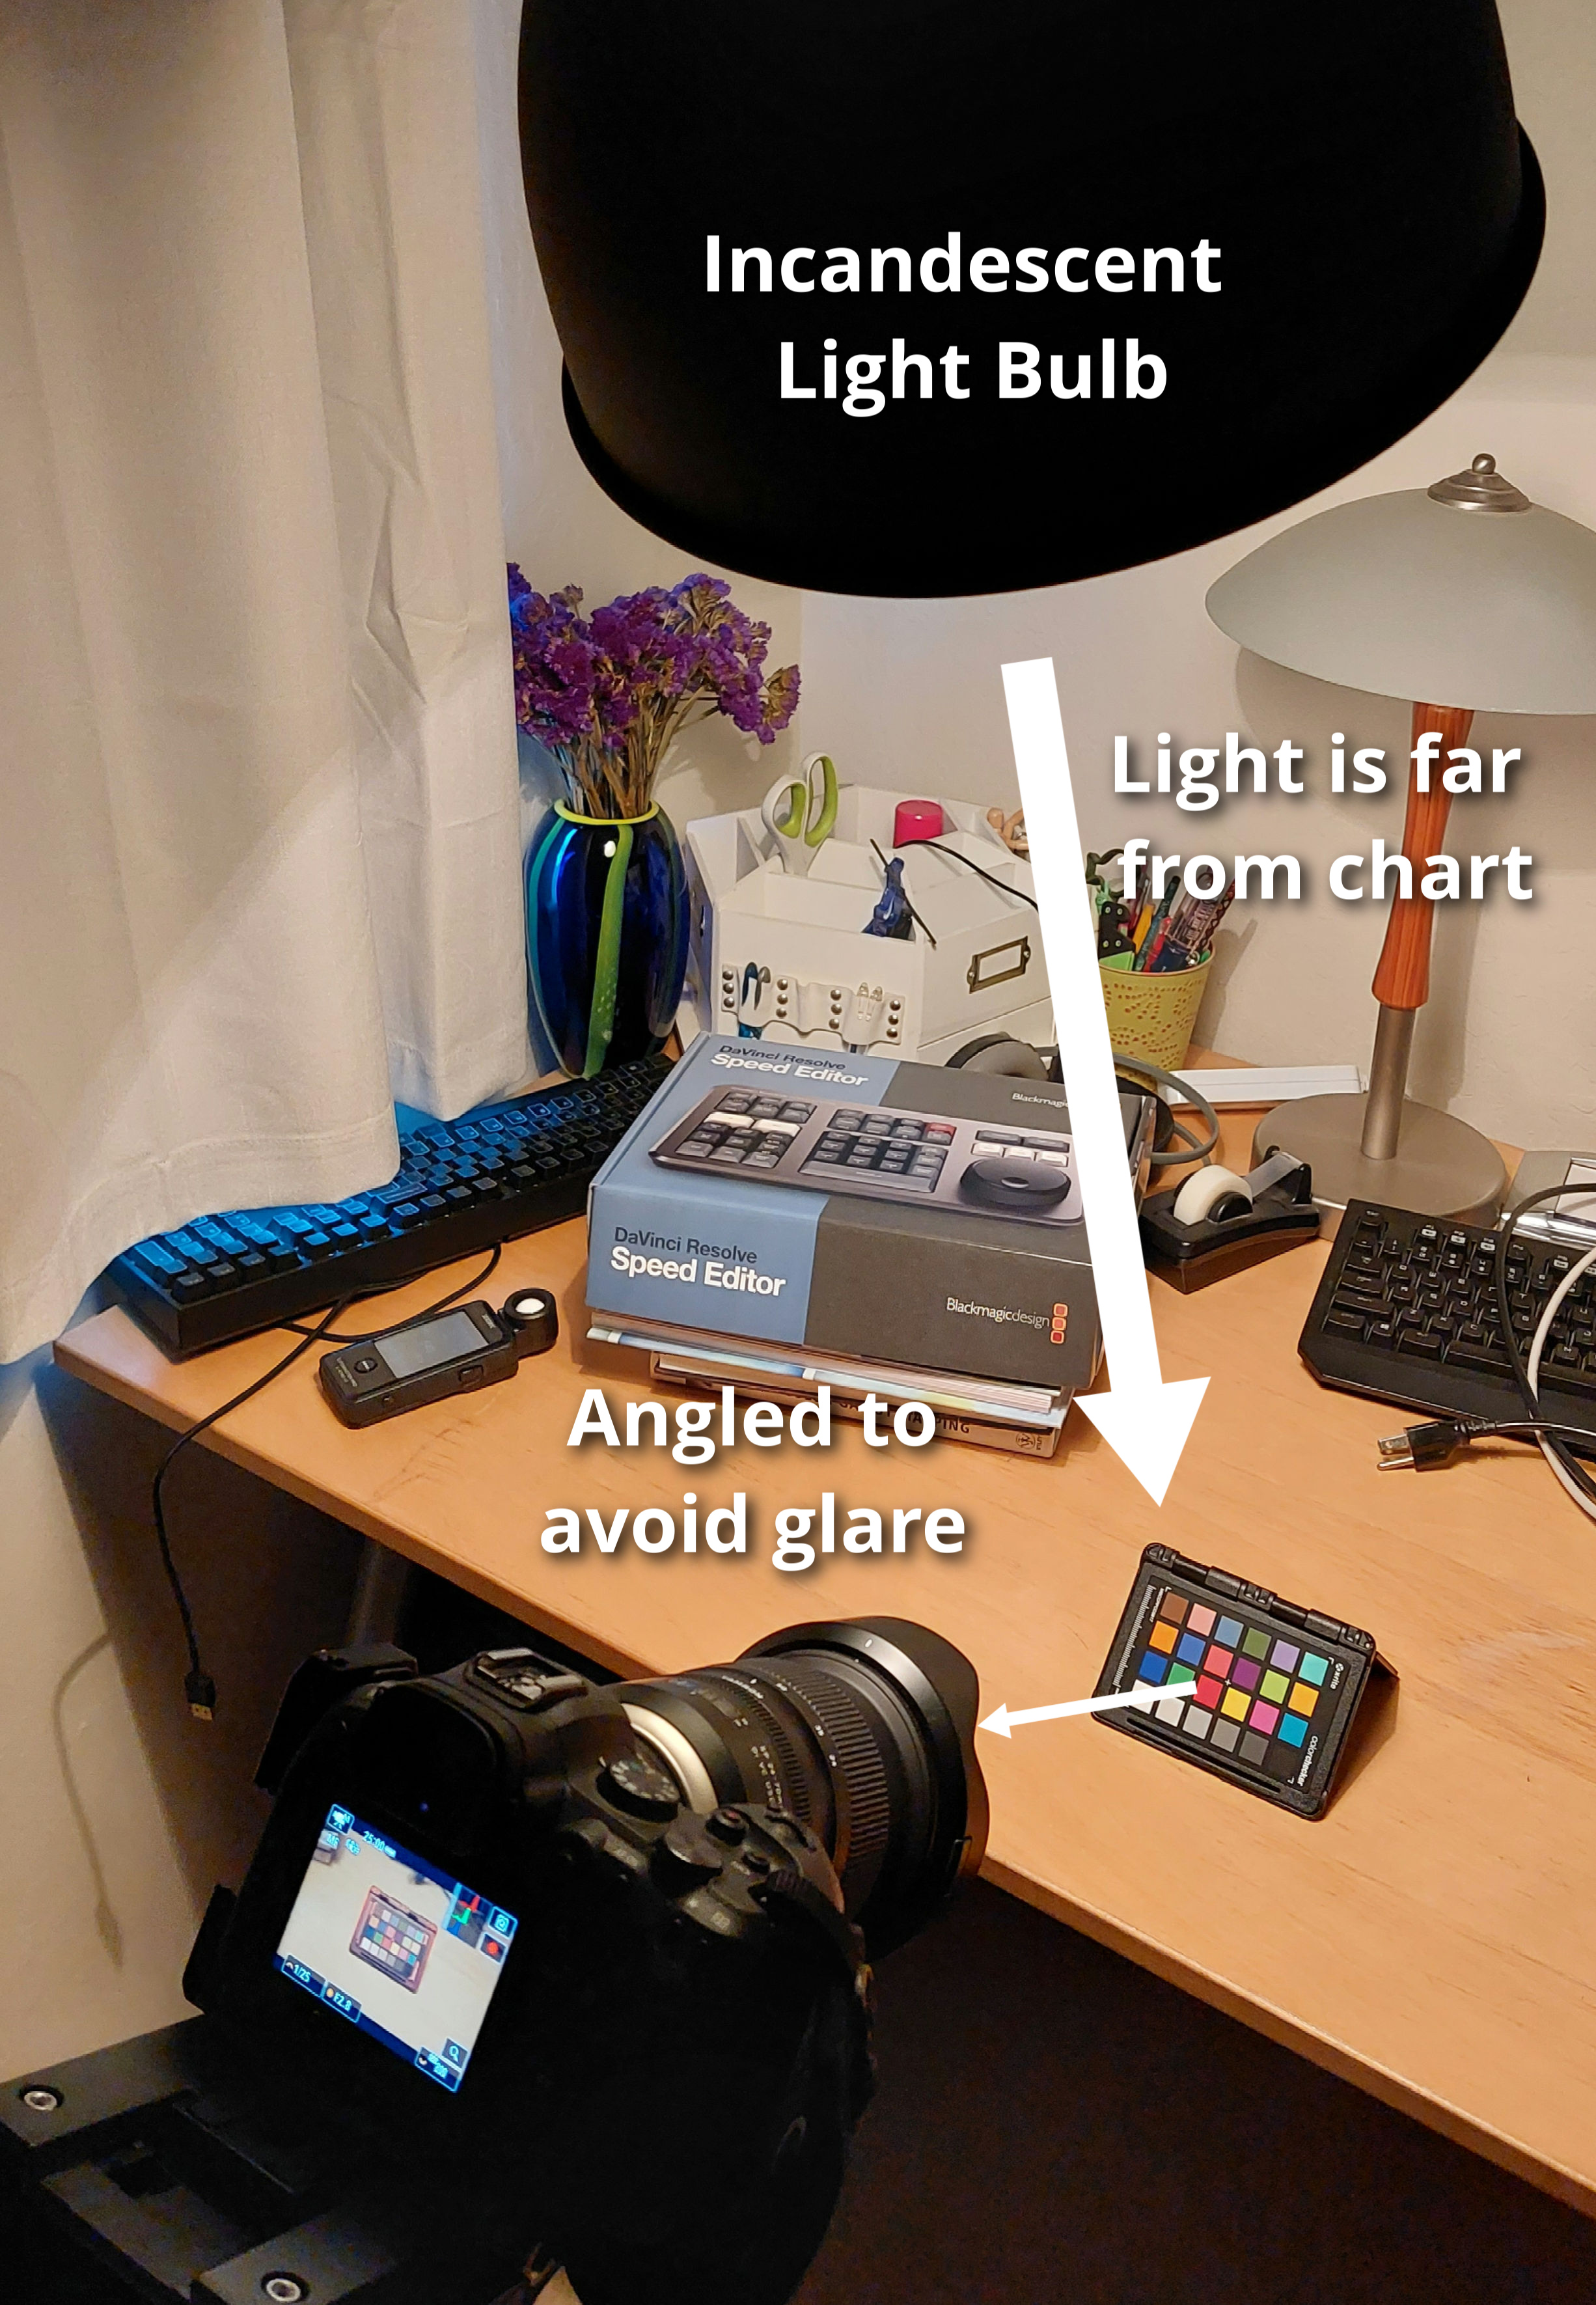
\includegraphics[scale=0.08]{images/tungsten_color_chart_setup0000.jpg}
\end{figure}

\subsubsection{Requirements}
\begin{enumerate}
    \item \textbf{Dark Background to control flaring} - We don't want there to be any lights or glares in the background of the image that would result in lens flaring.
    \item \textbf{Controlled Glare} - The light should be placed at such an angle to the color chart that the camera is not in-line with the primary reflection of the light in the color chart. IE if the color chart were a mirror, the light's reflection should not be visible to the camera. If the camera is normal to the test chart, putting the light at a 45 degree angle to the test chart would easily avoid this.
    \item \textbf{High quality light} - This test requires that you use an Incadescent light bulb rather than an LED light that merely simulates the illumination of a hot filament.
    \item \textbf{Correct White Balance} - The camera should be white balanced for this light source. Small discrepancies will be corrected via a small RGB gain adjustment, but the camera should be in the right ballpark for the shot.
    \item \textbf{Even lighting on the color chart} - Place the light farther from the test chart so that there aren't light fall-off problems (at least 4x the length of the long side of the test chart away).
    \item \textbf{Color chart fills the middle third of the image} - This is a compromise between maximizing the number of pixels we can sample for each color chip, and avoiding lens vignetting.
    \item \textbf{No light modifiers} - The bulb should not be covered by a lampshade or a softbox that may discolor the image, and likewise it should not be bounced off of colored walls.
\end{enumerate}

\subsection{White or Gray card under Standard Illuminant A}

\subsubsection{Procedure}
As this is merely to correct for any vignetting or lighting inconsistency in the color chart, this should be done under the same settings and lighting as in the previous image \ref{chartA}. The Color chart should be replaced by a neutrally colored card of about the same size.

\subsubsection{Requirements}
\begin{enumerate}
    \item \textbf{Same conditions as the shot of the Colorchecker under Std. Illuminant A} - We simply need to understand how consistent the lighting is on the color chart.
    \item \textbf{Uniformly colored card} - The card should not have marks or chips printed on it.
\end{enumerate}


\subsection{ColorChecker under Daylight}

\subsubsection{Procedure}
As with the Color Chart with Std. Illuminant A, we need to capture a shot of the color chart in direct sunlight. To avoid glare, the camera angle must be selected so that the main reflection from the sun is not in-line with the lens, and a dark background should be used behind the color chart.


\begin{figure}[ht]
    \centering
    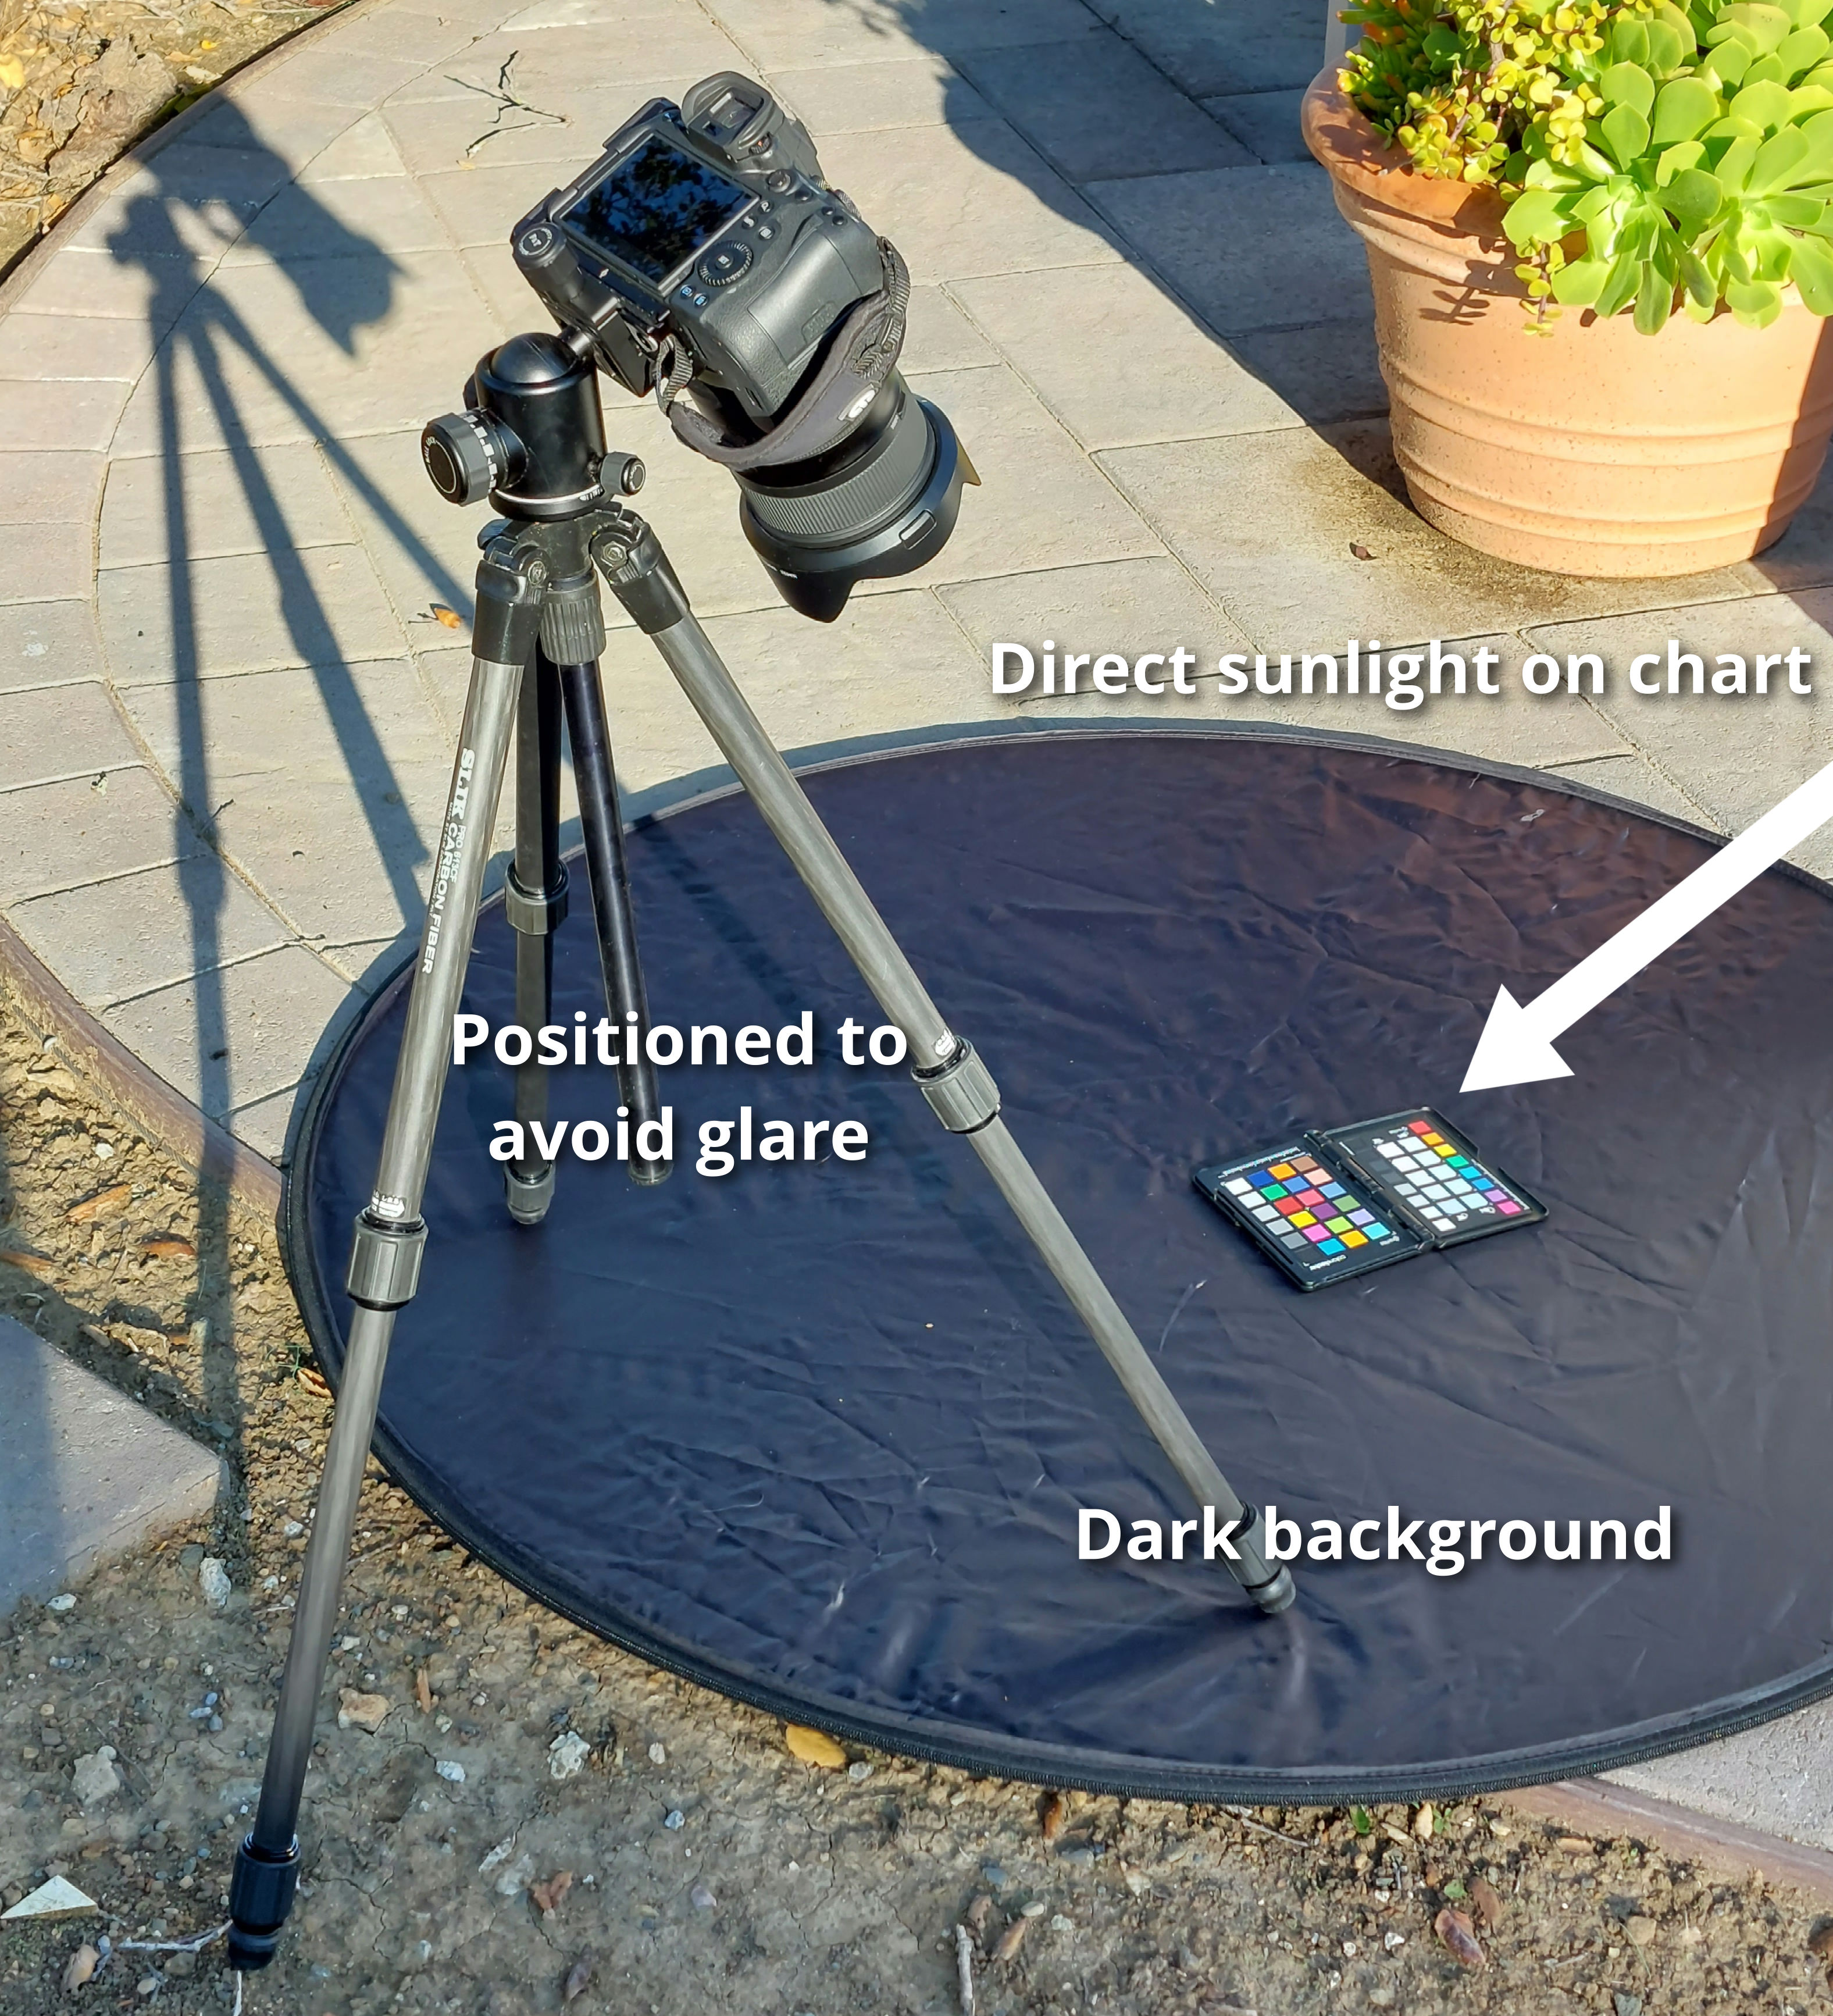
\includegraphics[scale=0.08]{images/sunlight_color_chart_setup0000.jpg}
\end{figure}

\subsubsection{Requirements}
\begin{enumerate}
    \item \textbf{Dark Background} - Lay down a black cloth or place the color checker on asphalt, etc.
    \item \textbf{Direct sunlight on the color chart} - The color chart should be hit directly by sunlight.
    \item \textbf{Even lighting on the color chart} - Avoid placing the color chart near objects that would reflect light onto the color chart, and avoid casting shadows on the chart.
    \item \textbf{Camera not in primary reflection of the sun} - Reduce glare by making sure the primary reflection of the sun in the color chart is not in the direction of the camera. This can be done by making sure the sun is front-lighting the color chart.
    \item \textbf{Time is afternoon or morning} - We ideally want to capture the color of the sun when it is neither sunset/sunrise/mid-day.
    \item \textbf{White Balance for daylight} - Set the camera's white balance to 5500K or Daylight, or a custom white balance for this sunlight.
\end{enumerate}

\subsection{White or Gray card under Daylight}
\subsubsection{Procedure}
Follow the same procedure as the ColorChecker under Daylight. The Color chart in the daylight shoot should be replaced with a uniform, neutrally colored card so that vignetting in the lens can be measured.

\subsubsection{Requirements}
\begin{enumerate}
    \item \textbf{Same conditions as the shot of the Colorchecker under Daylight} - Only interested in lens and lighting consistency on the color chart.
    \item \textbf{Uniformly colored card} - The card should not have marks or chips printed on it.
\end{enumerate}

%----------------------------------------------------------------------------------------

\end{document}
